
\begin{questions}

  
\question Translate into symbols.  Use $E(x)$ for ``$x$ is even'' and $O(x)$ for ``$x$ is odd.''
 \begin{parts}
  \part No number is both even and odd.
\part One more than any even number is an odd number.
\part There is prime number that is even.
\part Between any two numbers there is a third number.
\part There is no number between a number and one more than that number.
 \end{parts}

  \begin{answer}
     \begin{parts}
	\part $\neg \exists x (E(x) \wedge O(x))$
	\part $\forall x (E(x) \imp O(x+1))$
	\part $\exists x(P(x) \wedge E(x))$ (where $P(x)$ means ``$x$ is prime'')
	\part $\forall x \forall y \exists z(x < z < y \vee y < z < x)$
	\part $\forall x \neg \exists y (x < y < x+1)$
    \end{parts}
  \end{answer}

  
 
 
\question Translate into English:
\begin{parts}
 \part $\forall x (E(x) \imp E(x +2))$
\part $\forall x \exists y (\sin(x) = y)$
\part $\forall y \exists x (\sin(x) = y)$
\part $\forall x \forall y (x^3 = y^3 \imp x = y)$
\end{parts}

  \begin{answer}
    \begin{parts}
	\part Any even number plus 2 is an even number.
	\part For any $x$ there is a $y$ such that $\sin(x) = y$.  In other words, every number $x$ is in the domain of sine. 
	\part For every $y$ there is an $x$ such that $\sin(x) = y$.  In other words, every number $y$ is in the range of sine (which is false).
	\part For any numbers, if the cubes of two numbers are equal, then the numbers are equal.
      \end{parts}
  \end{answer}

  
  

\question Simplify the statements (so negation appears only directly next to predicates).
\begin{parts}
  \part $\neg \exists x \forall y (\neg O(x) \vee E(y))$
  \part $\neg \forall x \neg \forall y \neg(x < y \wedge \exists z (x < z \vee y < z))$
  \part There is a number $n$ for which no other number is either less $n$ than or equal to $n$.
  \part It is false that for every number $n$ there are two other numbers which $n$ is between.
\end{parts}

  \begin{answer}
    \begin{parts}
	\part $\forall x \exists y (O(x) \wedge \neg E(y))$
	\part $\exists x \forall y (x \ge y \vee \forall z (x \ge z \wedge y \ge z))$
	\part There is a number $n$ for which every other number is strictly greater than $n$.
	\part There is a number $n$ which is not between any other two numbers.
      \end{parts}
  \end{answer}

  
\question Let $A = \{1,2,3,4,5\}$, $B = \{3,4,5,6,7\}$ and $C = \{2,3,5\}$.
\begin{parts}
 \part Find $A \cap B$.
 \part Find $A \cup B$.
 \part Find $A \setminus B$.
 \part Is $C \subseteq A$?
 \part Is $C \subseteq B$?
\end{parts}

  \begin{answer}
    \begin{parts}
	\part $A \cap B = \{3,4,5\}$.  %Find $A \cap B$.
	\part $A \cup B = \{1,2,3,4,5,6,7\}$. %Find $A \cup B$.
	\part $A \setminus B = \{1,2\}$. %Find $A \setminus B$.
	\part Yes.  %Is $C \subseteq A$?
	\part No. %Is $C \subseteq B$?
    \end{parts}
  \end{answer}

  

\question Let $A = \{x \in \N \st 3 \le x \le 13\}$, $B = \{x \in \N \st x \mbox{ is even}\}$, and $C = \{x \in \N \st x \mbox{ is odd}\}$.
\begin{parts}
  \part Find $A \cap B$.
  \part Find $A \cup B$.
  \part Find $B \cap C$.
  \part Find $B \cup C$.
\end{parts}

  \begin{answer}
    \begin{parts}
  %Find $A \cap B$
	\part $A \cap B = \{4,6,8,10,12\}$
  % Find $A \cup B$.
	\part $A \cup B = \{x \in \N \st (3 \le x \le 13) \vee x \mbox{ is even}\}.$ (the set of all natural numbers which are either even or between 3 and 13 inclusive).
  %Find $B \cap C$.
	\part $B \cap C = \emptyset$.
  %Find $B \cup C$.
	\part $B \cup C = \N$.
      \end{parts}
  \end{answer}



\question Find an example of sets $A$ and $B$ such that $A\cap B = \{3, 5\}$ and $A \cup B = \{2, 3, 5, 7, 8\}$.

  \begin{answer}
    For example, $A = \{2,3,5,7,8\}$ and $B = \{3,5\}$.
  \end{answer}



\question Find an example of sets $A$ and $B$ such that $A \subseteq B$ and $A \in B$.

  \begin{answer}
    Let $A = \{1,2,3\}$ and $B = \{1,2,3,4,5,\{1,2,3\}\}$
  \end{answer}

  

\question Recall $\Z = \{\ldots,-2,-1,0, 1,2,\ldots\}$ (the integers).  Let $\Z^+$ be the positive integers.  Let $2\Z$ be the even integers, $3\Z$ be the multiples of 3, and so on.
\begin{parts}
  \part Is $\Z^+ \subseteq 2\Z$?  
  \part Is $2\Z \subseteq \Z^+$?  
  \part Find $2\Z \cap 3\Z$.  Describe the set in words, and also in symbols (using a $\st$ symbol).
  \part Express $\{x \in \Z \st \exists y\in \Z (x = 2y \vee x = 3y)\}$ as a union or intersection of two sets above.
\end{parts}

  \begin{answer}
    \begin{parts}
	\part No.
	\part No.
	\part $2\Z \cap 3\Z$ is the set of all integers which are multiples of both 2 and 3 (so multiples of 6).  Therefore $2\Z \cap 3\Z = \{x \in \Z \st \exists y\in \Z(x = 6y)\}$.
	\part $2\Z \cup 3\Z$.
 \end{parts}
  \end{answer}



\question Let $A_2$ be the set of all multiples of 2 except for $2$.  Let $A_3$ be the set of all multiples of 3 except for 3.  And so on, so that $A_n$ is the set of all multiple of $n$ except for $n$, for any $n \ge 2$.  Describe (in words) the set $\bar{A_2 \cup A_3 \cup A_4 \cup \cdots}$

  \begin{answer}
    The set of primes.
  \end{answer}




\question Draw a Venn diagram to represent each of the following:
\begin{parts}
 \part $A \cup \bar B$
 \part $\bar{(A \cup B)}$
 \part $A \cap (B \cup C)$
 \part $(A \cap B) \cup C$
 \part $\bar A \cap B \cap \bar C$
 \part $(A \cup B) \setminus C$
\end{parts}

  \begin{answer}	  
%  \begin{multicols}{3}
      \begin{parts}
	  \def\circleA{(-.5,0) circle (1)}
	  \def\circleAlabel{(-1.5,.6) node[above]{$A$}}
	  \def\circleB{(.5,0) circle (1)}
	  \def\circleBlabel{(1.5,.6) node[above]{$B$}}
	  \def\circleC{(0,-1) circle (1)}
	  \def\circleClabel{(.5,-2) node[right]{$C$}}
	  \def\twosetbox{(-2,-1.5) rectangle (2,1.5)}
	  \def\threesetbox{(-2,-2.5) rectangle (2,1.5)}
	  

	  
	    \part  $A \cup \bar B$:
	    
	    \begin{tikzpicture}[fill=gray!50]
	  %Fill A:
	  \fill \circleA;
	  %Fill \bar B:
	    \begin{scope}
	    \clip \circleB \twosetbox; %This defines the scope to everything in the twosetbox which is not in circleB.
	    \fill \twosetbox;
	    \end{scope}
	    \draw[thick] \circleA \circleAlabel \circleB \circleBlabel \twosetbox;
	  \end{tikzpicture}


	  %   
	  \part $\bar{(A \cup B)}$:

	  \begin{tikzpicture}[fill=gray!50]
	    \fill \twosetbox;
	    \fill[white] \circleA \circleB;
	    \draw[thick] \circleA \circleAlabel \circleB \circleBlabel \twosetbox;
	  \end{tikzpicture}

%	  \columnbreak

	  %   
	  \part $A \cap (B \cup C)$:

	  \begin{tikzpicture}[fill=gray!50]
	  \begin{scope}
	    \clip \circleA;
	    \fill \circleB \circleC;
	  \end{scope}
	  \draw[thick] \circleA \circleAlabel \circleB \circleBlabel \circleC \circleClabel \threesetbox;
	  \end{tikzpicture}

	  %  
	  \part $(A \cap B) \cup C$:

	  \begin{tikzpicture}[fill=gray!50]
	  \begin{scope}
	    \clip \circleA;
	    \fill \circleB;
	  \end{scope}
	  \fill \circleC;
	  \draw[thick] \circleA \circleAlabel \circleB \circleBlabel \circleC \circleClabel \threesetbox;
	  \end{tikzpicture}

	 
%	  \columnbreak
	  %   
	  \part $\bar A \cap B \cap \bar C$:

	  \begin{tikzpicture}[fill=gray!50]
	  \fill \circleB;
	  \begin{scope}
	    \clip \circleB;
	    \fill[white] \circleA \circleC;
	  \end{scope}

	  \draw[thick] \circleA \circleAlabel \circleB \circleBlabel \circleC \circleClabel \threesetbox;
	  \end{tikzpicture}

	  %   
	  \part $(A \cup B) \setminus C$:

	  \begin{tikzpicture}[fill=gray!50]
	  \fill \circleA;
	  \fill \circleB;
	  \fill[white] \circleC;
	  \draw[thick] \circleA \circleAlabel \circleB \circleBlabel \circleC \circleClabel \threesetbox;
	  \end{tikzpicture}

	  \end{parts}	 
%	   \end{multicols}
  \end{answer}




\question Describe a set in terms of $A$ and $B$ which has the following Venn diagram:

\begin{center}
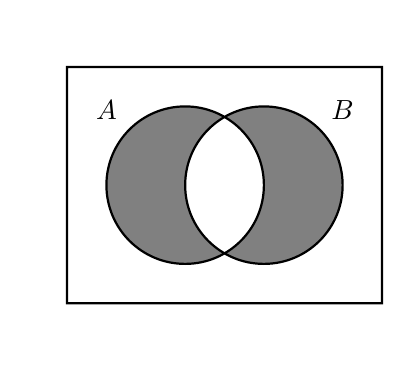
\begin{tikzpicture}[fill=gray]
% left hand
\scope
\clip (-2,-2) rectangle (2,2)
      (1,0) circle (1);
\fill (0,0) circle (1);
\endscope
% right hand
\scope
\clip (-2,-2) rectangle (2,2)
      (0,0) circle (1);
\fill (1,0) circle (1);
\endscope
% outline
\draw[thick] (0,0) circle (1) (-1,.7)  node [text=black,above] {$A$}
      (1,0) circle (1) (2,.7)  node [text=black,above] {$B$}
      (-1.5,-1.5) rectangle (2.5,1.5);
\end{tikzpicture}
\end{center}

  \begin{answer}
    For example, $A \cup B \cap \bar{(A \cap B)}$.  Note that $\bar{A \cap B}$ would almost work, but also contain the area outside of both circles.
  \end{answer}

  

\question Find the cardinalities:
\begin{parts}
  \part Find $|A|$ when $A = \{4,5,6,\ldots,37\}$
  \part Find $|A|$ when $A = \{x \in \Z \st -2 \le x \le 100\}$
  \part Find $|A \cap B|$ when $A = \{x \in \N \st x \le 20\}$ and $B = \{x \in \N \st x \mbox{ is prime}\}$
\end{parts}

  \begin{answer}
      \begin{parts}
	  \part 34.
	  \part 103.
	  \part 8.
      \end{parts}
  \end{answer}


  
  
\question Let $A = \{a, b, c\}$.  Find $\pow(A)$.

  \begin{answer}
    $\pow(A) = \{\emptyset, \{a\}, \{b\}, \{c\}, \{a,b\}, \{a,c\}, \{b,c\}, \{a,b,c\}\}$.
  \end{answer}

  
  

\question Let $A = \{1,2,\ldots, 10\}$.  How many subsets of $A$ contain exactly one element (i.e., how many {\em singleton} subsets are there).  How many {\em doubleton} (containing exactly two elements) are there?

  \begin{answer}
      There are 10 singletons.  There are 45 doubletons (because $45 = 9+8+7+\cdots+2+1$).
  \end{answer}


  
  
\question Let $A = \{1,2,3,4,5,6\}$.  Find all sets $B \in \pow(A)$ which have the property $\{2,3,5\} \subseteq B$.

  \begin{answer}
      $\{2,3,5\}, \{1,2,3,5\}, \{2,3,4,5\}, \{2,3,5,6\}, \{1,2,3,4,5\}, \{1,2,3,5,6\}, \{2,3,4,5,6\}$, and $\{1,2,3,4,5,6\}$.
  \end{answer}


  
\question Find an example of sets $A$ and $B$ such that $|A| = 4$, $|B| = 5$ and $|A \cup B| = 9$.  

  \begin{answer}
   For example $A = \{1,2,3,4\}$ and $B = \{5,6,7,8,9\}$.
  \end{answer}

  
  

\question Find an example of sets $A$ and $B$ such that $|A| = 3$, $|B| = 4$ and $|A \cup B| = 5$.

  \begin{answer}
    For example, $A = \{1,2,3\}$ and $B = \{2,3,4,5\}$.
  \end{answer}



\question In a regular deck of playing cards there are 26 red cards and 12 face cards.  Explain in terms of sets why there are only 32 cards which are either red or a face card.

  \begin{answer}
      If $R$ is the set of red cards and $F$ is the set of face cards, we want to find $|R \cup F|$.  This is not simply $|R| + |F|$ because there are 6 cards which are both red and a face card; $|R \cap F| = 6$.  We find $|R \cup F| = 32$.
  \end{answer}


  
% \question A group of college students were asked about their TV watching habits.  Of those surveyed, 28 students watch {\em House}, 19 watch {\em Castle} and 24 watch re-runs of {\em 24}.  Additionally, 16 watch {\em House} and {\em Castle}, 14 watch {\em House} and {\em 24} and 10 watch {\em Castle} and {\em 24}.  There are 8 students who watch all three shows.  How many students surveyed watched at least one of the shows?
% 
%   \begin{answer}
%     39.
%   \end{answer}
% 
% 
% 
% \question Find $|(A \cup C)\cap \bar B|$ provided $|A| = 50$, $|B| = 45$, $|C| = 40$, $|A\cap B| = 20$, $|A \cap C| = 15$, $|B \cap C| = 23$ and $|A \cap B \cap C| = 12$.
% 
%     \begin{answer}
%       $|(A \cup C)\cap \bar B| = 44$
%     \end{answer}
% 
% 
% 
% \question Using the same data as the previous question, describe a set with cardinality 26.
% 
%     \begin{answer}
% 	One possibility: $(A \cup B) \cap C$.
%     \end{answer}



  

% \question Consider the statement ``for all integers $a$ and $b$, if $a + b$ is even, then $a$ and $b$ are even''
% \begin{parts}
%  \part Write the contrapositive of the statement
%  \part Write the converse of the statement
%  \part Write the negation of the statement.
%  \part Is the original statement true or false?  Prove your answer.
%  \part Is the contrapositive of the original statement true or false?  Prove your answer.
%  \part Is the converse of the original statement true or false?  Prove your answer.
%  \part Is the negation of the original statement true or false?  Prove your answer.
% \end{parts}
% 
%   \begin{answer}
%     \begin{parts}
% 	\part For all integers $a$ and $b$, if $a$ or $b$ are not even, then $a+b$ is not even.
% 	\part For all integers $a$ and $b$, if $a$ and $b$ are even, then $a+b$ is even.
% 	\part There are numbers $a$ and $b$ such that $a+b$ is even but $a$ and $b$ are not both even.
% 	\part False.  For example, $a = 3$ and $b = 5$.  $a+b = 8$, but neither $a$ nor $b$ are even.
% 	\part False, since it is equivalent to the original statement.
% 	\part True.  Let $a$ and $b$ be integers.  Assume both are even.  Then $a = 2k$ and $b = 2j$ for some integers $k$ and $j$.  But then $a+b = 2k + 2j = 2(k+j)$ which is even.
% 	\part True, since the statement is false.
%       \end{parts}
%   \end{answer}
% 
% 
%   
%   
% \question Prove that $\sqrt 3$ is irrational.
% 
%   \begin{answer}
%     \begin{proof}
%      Suppose $\sqrt{3}$ were rational.  Then $\sqrt{3} = \frac{a}{b}$ for some integers $a$ and $b \ne 0$.  Without loss of generality, assume $\frac{a}{b}$ is reduced.  Now
% \[3 = \frac{a^2}{b^2}\]
% \[b^2 3 = a^2\]
% So $a^2$ is a multiple of 3.  This can only happen if $a$ is a multiple of 3, so $a = 3k$ for some integer $k$.  Then we have
% \[b^2 3 = 9k^2\]
% \[b^2 = 3k^2\]
% So $b^2$ is a multiple of 3, making $b$ a multiple of 3 as well.  But this contradicts our assumption that $\frac{a}{b}$ is in lowest terms.
%     \end{proof}
%   \end{answer}

 
 
 
\end{questions}





